\documentclass[11px, a4paper, twocolumn]{article}

\usepackage[utf8]{inputenc}
\usepackage[swedish]{babel}

\usepackage{graphicx}
\usepackage{epstopdf}
\usepackage{color}
\usepackage[final]{pdfpages}
\usepackage{subfigure}
\usepackage{float}
\usepackage{caption}
\usepackage{epigraph}
\usepackage{wrapfig}



\usepackage[hyphens]{url}
\usepackage[breaklinks,pdfpagelabels=false]{hyperref}


% Mail link
\newcommand{\mail}[1]{\href{mailto:#1}{\nolinkurl{#1}}}

\addto{\captionsswedish}{\renewcommand{\abstractname}{}}

\renewcommand{\familydefault}{\sfdefault}

\setlength{\epigraphwidth}{0.48\textwidth}


\hypersetup{
    pdftitle={Picture Hunter},
    pdfauthor={Daniel Ström},
    colorlinks=true,
    citecolor=magenta,
    filecolor=magenta,
    linkcolor=black,
    urlcolor=magenta
}


\title{Picture Hunter}
\author{Daniel Ström \\ \mail{D@nielstrom.se}}

\begin{document}

\maketitle
	
\epigraph{%
	Picture Hunter är ett spel för dig som inte bara vill sitta hemma och pula. Spelet tar dig ut i världen mot nya upplevelser tillsammans med en eller flera vänner. Uppdraget: att hitta de andra spelarnas gömda platser enbart utifrån ett fotografi och en grov idé om vart det kan ha tagits.%
}{\sc{Beskrivning på Google Play}}

\tableofcontents

\listoffigures


\section{Introduktion}
	Picture hunter kan liknas vid en modern smartphone-variant på leken ``Följa John''. Idén är att en spelare tar ett kort på något och sedan skickar kortet till en annan spelare. Den andra spelarens uppgift är att försöka ta samma kort och därigenom ``matcha'' det.

	Ett grundläggande scenario för appens användande har varit att upptäcka en stad. I detta fall ger två personer varandra bilder de tagit någonstanns i staden. För att underlätta detta kan användaren se hur långt bort bilden är tagen (men inte vilken riktning; det är ju ett spel trots allt).

	Min ambition för appen är att den ska vara bra nog för ett VG men då jag har begränsat med tid till återinlämningar nöjer jag mig med ett G om det inte rör sig om mycket små förändringar som erfodras för att nå det högre betyget.


\section{Design}

	Interaktionen i appen utgörs av tre distinkta aktiviteter: filhantering, bildjämförelse,	bilddelning. Målet för designen av dessa aktiviteter är att skapa en homogen upplevelse som passar in med androids övriga utseende. Dessutom försöker appen vara så transparent som möjligt. Fokus för användaren ska ligga på att försöka hitta bilden, inte på att navigera appen. Som en följd av detta försöker Picture Hunter inte fånga användarens uppmärksammhet genom starka färger i gränssnittet utan använder i den mån det är möjligt standardutseendet för kontroller och ikoner. Då ikoner inte funnits har nya skapats i motsvarande stil.

	De tre aktiviteterna nämnda ovan har delats upp i två olika gränssnitt Det första sköter både filhantering och bilddelning, det andra hanterar bildjämförelse.

lbums
\subsection{Filhantering och delning}

	Denna del av appen fungerar i huvudsak som en filhanterare begränsad till appens externa lagringsutrymme. Lagringsutrymmet utgörs inte av appens privata utrymme utan består av en mapp som är nåbara av alla applikationer och som inte tas bort automatiskt vid avinstallering av appen. Detta val är gjort som en följd av designprincipen ``Never lose my stuff''\cite{Principles}.

	\begin{figure}[p]
		\centering
	    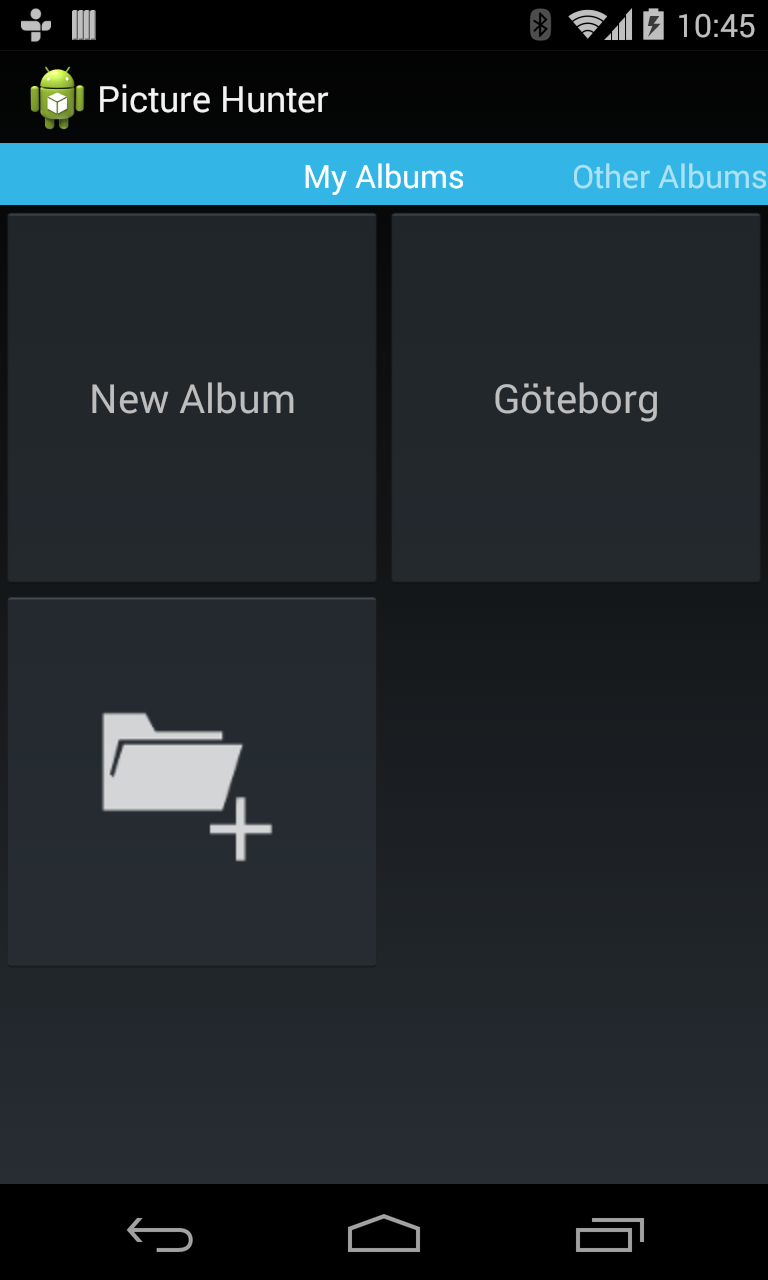
\includegraphics[width=0.3\textwidth]{img/albums}
		\caption{\label{fig:albums} Album med användarens egna bilder.}
	\end{figure}

	\begin{figure}[p]
		\centering
	    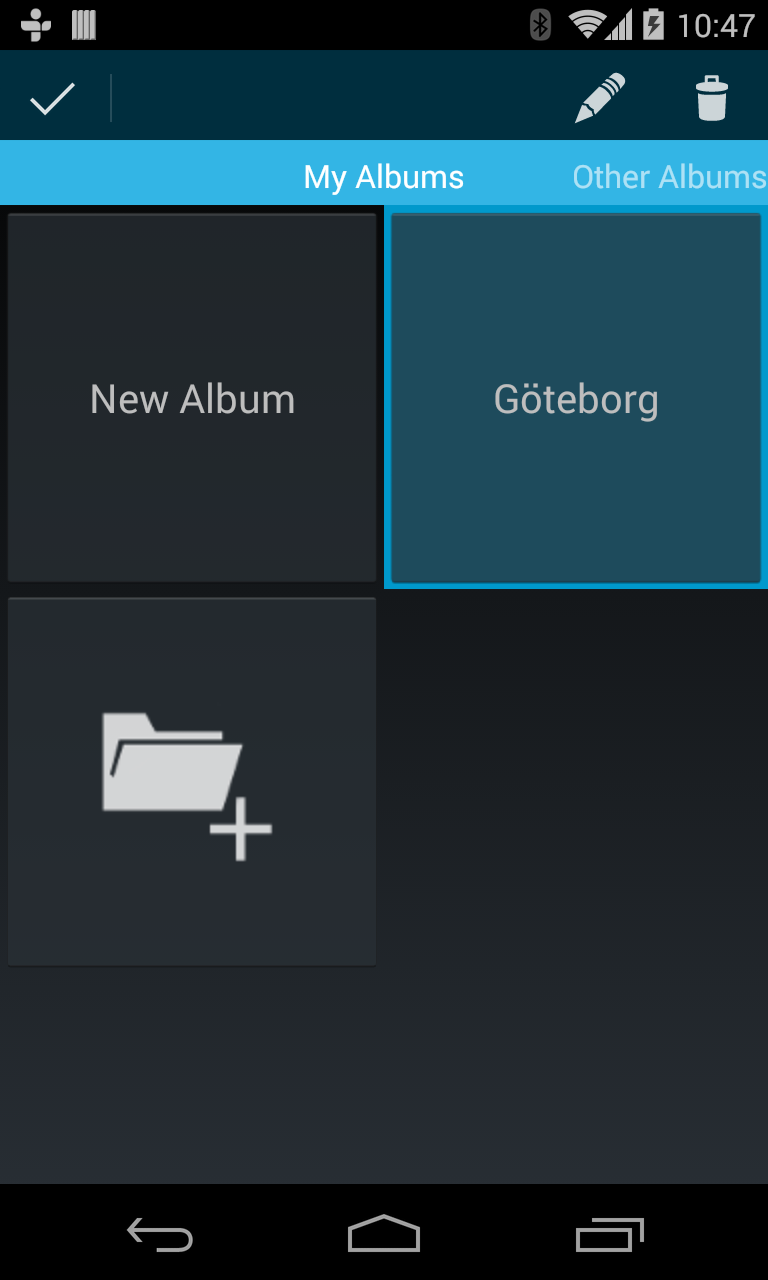
\includegraphics[width=0.3\textwidth]{img/albums_selection}
		\caption{\label{fig:albums_selection}Kontextknappar visas när man valt ett album.}
	\end{figure}

	Filhanteringen sker i två lager. Det första lagret hanterar ``album'' - sammlingar av bilder. Detta lagret kan ses i figur \ref{fig:albums}. Ett nytt album skapas genom att man klickar på ikonen med en mapp och ett plusstecken. Om man markerar en app genom att hålla ner fingret på den en kort tid visas en ny \emph{ActionBar}\cite{ContextActionBar} som ger möjligheten att byta namn eller ta bort albumet (se figur \ref{fig:albums_selection}). Detta följer androids designprincip ``Only show what I need when I need it''\cite{Principles}. Omdöpning av album görs med hjälp av en dialogruta anpassad för ändamålet. Vid borttagning av album visas också en dialogruta där användaren måste bekräfta valet\cite{Dialogs}. Dialogrutorna kan ses i figur \ref{fig:albums_selection_rename} och figur \ref{fig:albums_selection_delete}.

	\begin{figure}[p]
		\centering
	    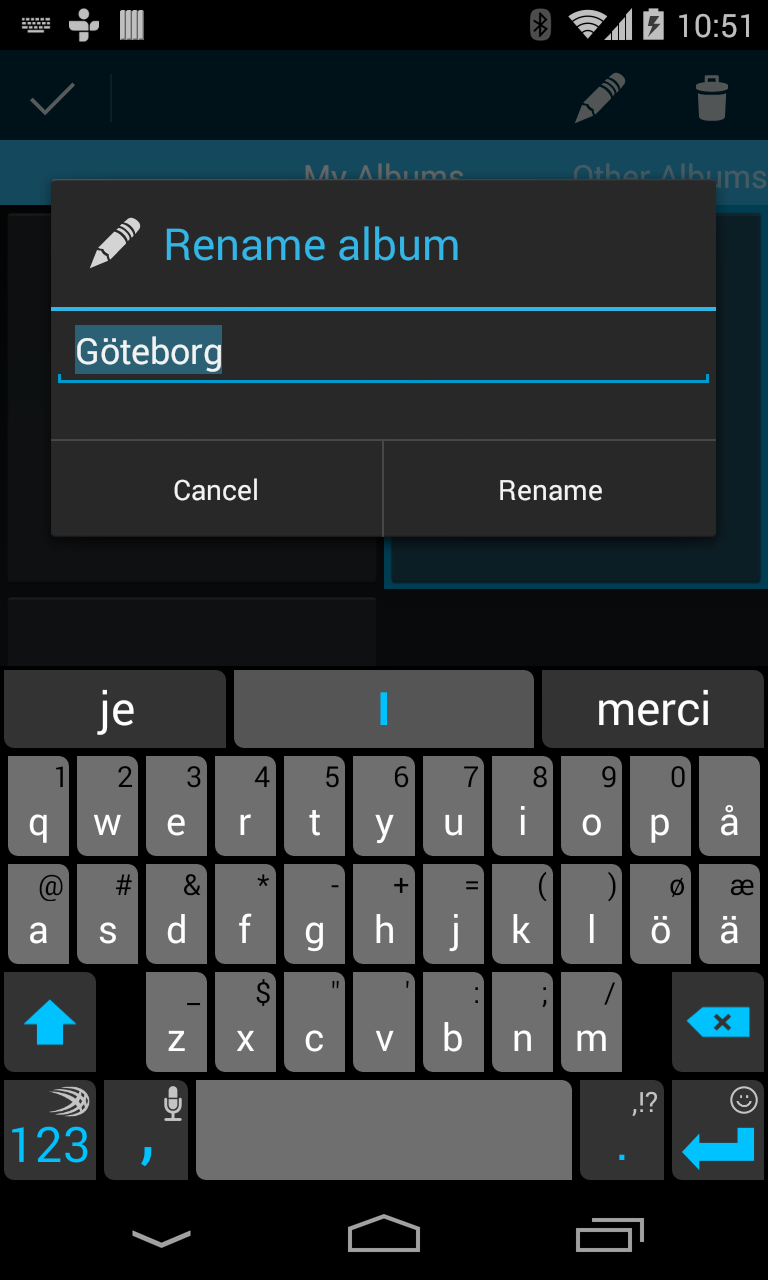
\includegraphics[width=0.3\textwidth]{img/albums_selection_rename}
		\caption{\label{fig:albums_selection_rename}En specialgjord dialog öppnas för att döpa om filer och album.}
	\end{figure}

	\begin{figure}[p]
		\centering
	    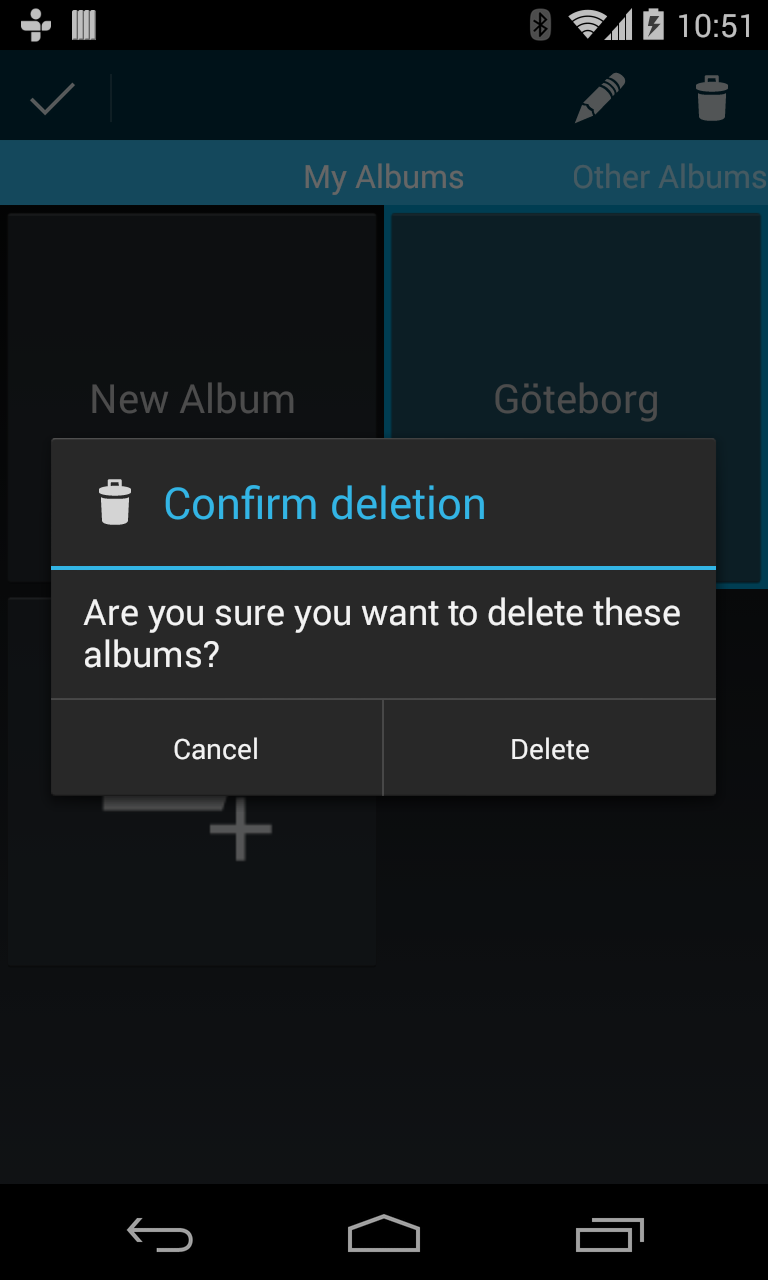
\includegraphics[width=0.3\textwidth]{img/albums_selection_delete}
		\caption{\label{fig:albums_selection_delete}För att ta bort saker måste användaren bekräfta handlingen.}
	\end{figure}

	Förutom de olika albumen finns två olika typer av album - egna album och främmande album. Egna album är album med bilder du tagit. Främmande album innehåller bilder du ska försöka matcha. De olika typerna av album presenteras i en horisontellt paginerad lista som rekomenderas för navigering bland kategorier\cite{HorizontalPaging}. För att användaren inte ska tappa bort vart hen befinner sig skrivs den nuvarande positionen ut i det ljusblå bandet ovanför listan med album (uppfyller designprincip ``I should always know where I am''\cite{Principles} ).


	\begin{figure}[p]
		\centering
	    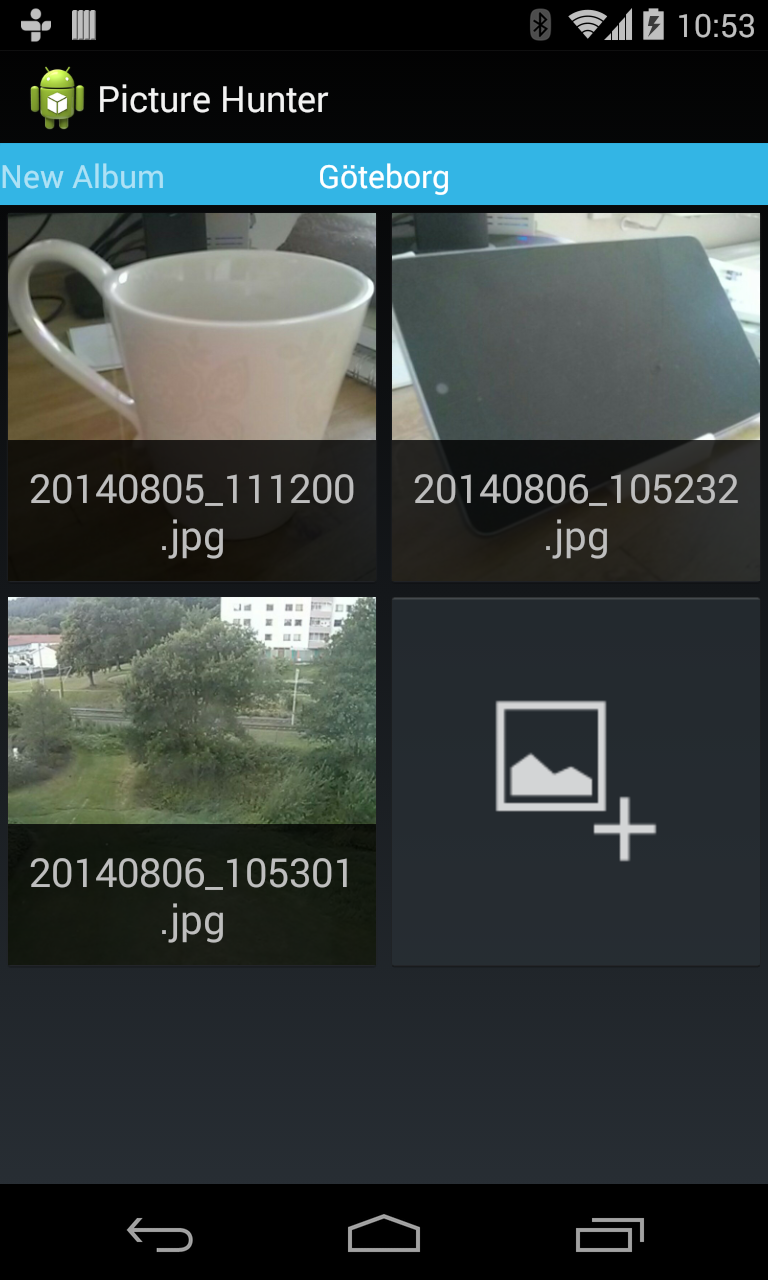
\includegraphics[width=0.3\textwidth]{img/photos}
		\caption{\label{fig:photos}Foton visas som miniatyrer.}
	\end{figure}

	\begin{figure}[p]
		\centering
	    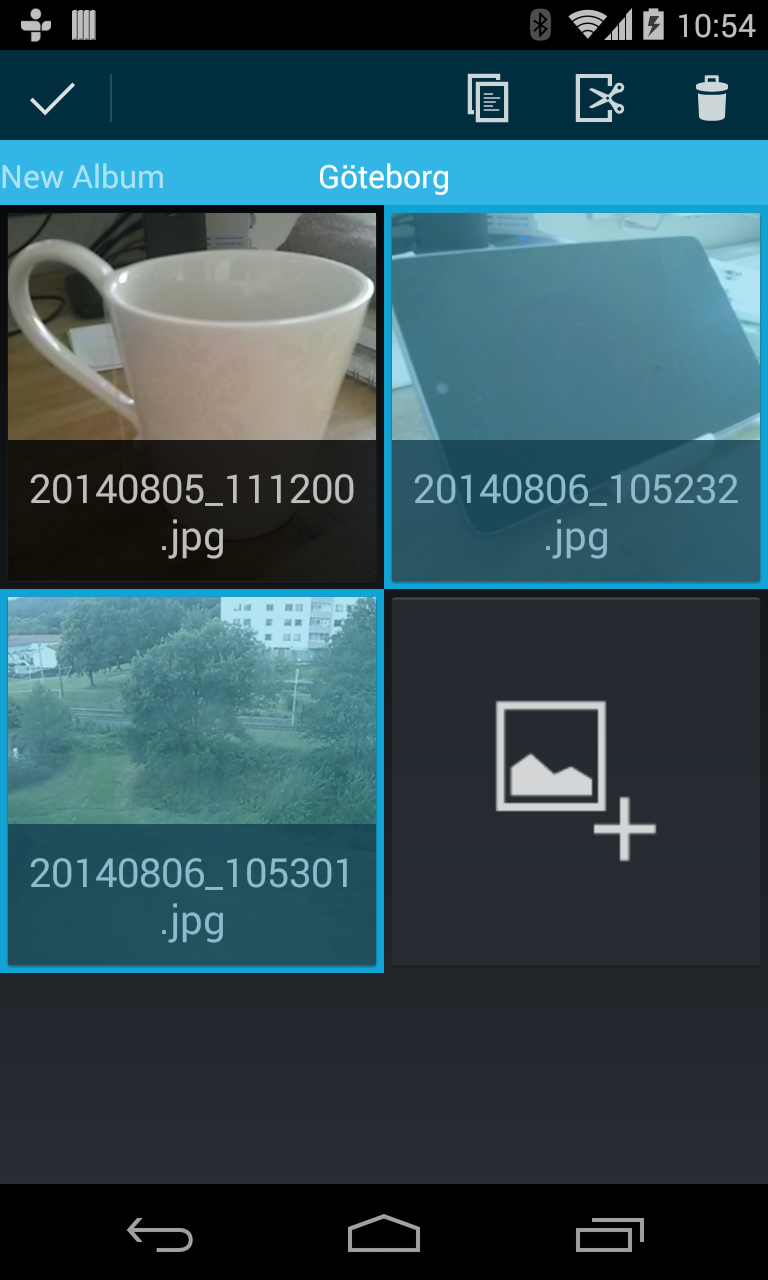
\includegraphics[width=0.3\textwidth]{img/photos_selection}
		\caption{\label{fig:photos_selection}Foton kan även kopieras och klippas ut.}
	\end{figure}

	\begin{figure}[p]
		\centering
	    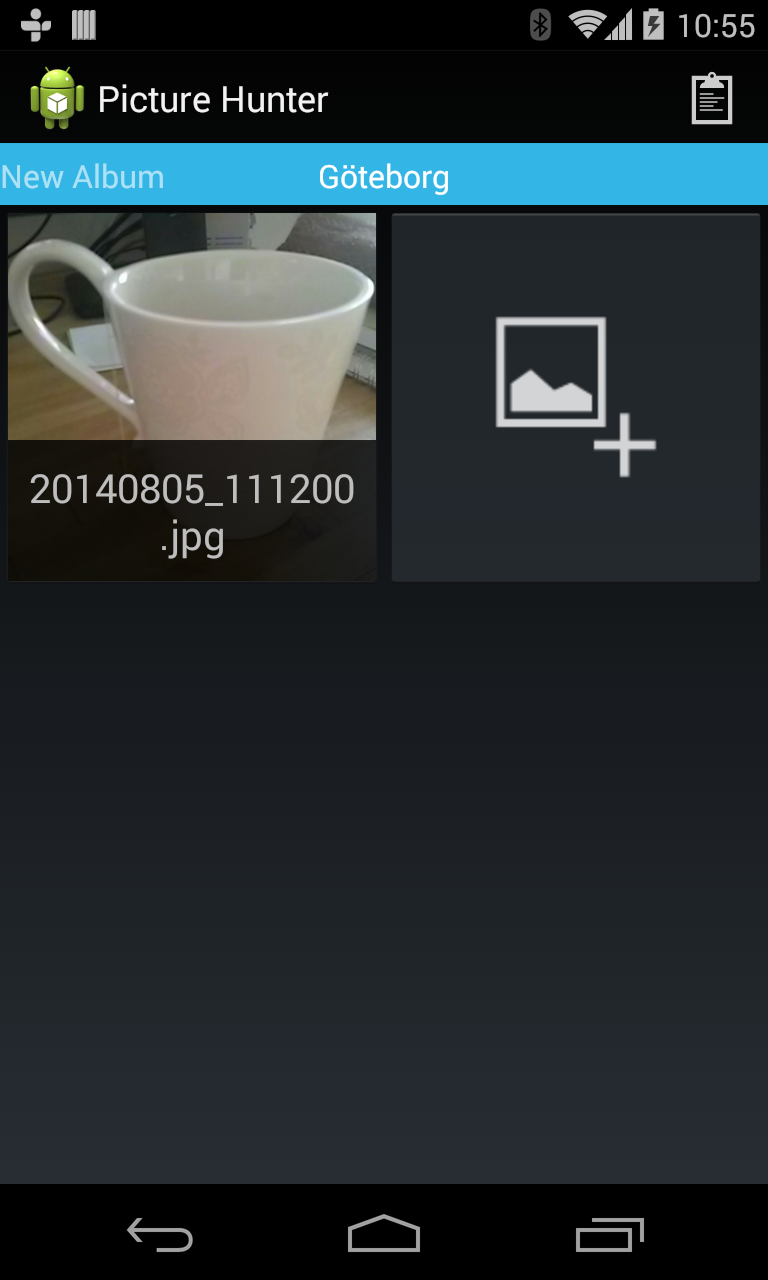
\includegraphics[width=0.3\textwidth]{img/photos_paste}
		\caption{\label{fig:photos_paste}Med bilder i utklippet visas en klistra-in knapp.}
	\end{figure}

	Figur \ref{fig:photos} visar det andra lagret. Detta lager visar bilderna som miniatyrer med deras namn i ett band längst ner (designprincip ``Pictures are faster than words''\cite{Principles}). Även här kan man markera i listan genom att hålla ner fingret. Här ges dock även möjligheten att kopiera eller klippa ut bilderna (se figur \ref{fig:photos_selection}). Ifall något har kopierats visas en klistra-in ikon i den normala ActionBar:en (figur \ref{fig:photos_paste}).

	Ifall användaren håller upp sin telefon mot en annan (som har samma app installerad och vars skärm är upplåst) medans bilder är markerade, skickas dessa till den andra telefonen. Telefonen som tar emot bilderna kommer få en notifikation av Android Beam när filerna är överförda och klickar man på notifikationen öppnas appen automatiskt till ett nytt album som innehåller bilderna.

	Nästan alla ikoner har hämtats från Androids bibliotek för ActionBar ikoner\cite{Icons}. Enda undantaget är ``Nytt Album''-ikonen som är en anpassad version av ``Collections''-ikonen.

	Båda dessa gränssnitt använder horisontell navigering mellan syskon-mappar (dvs. Mina album/Främmande album eller Album 1/Album 2/...). Användaren undviker på detta sätt upp till 50\% av knapptryckningarna som hade behövts om hen behövt backa ett steg för att nå ett syskon. Dessutom uppfyller navigationen designprincipen ``Give me tricks that work everywhere''\cite{Principles}.

	\begin{figure}[p]
		\centering
	    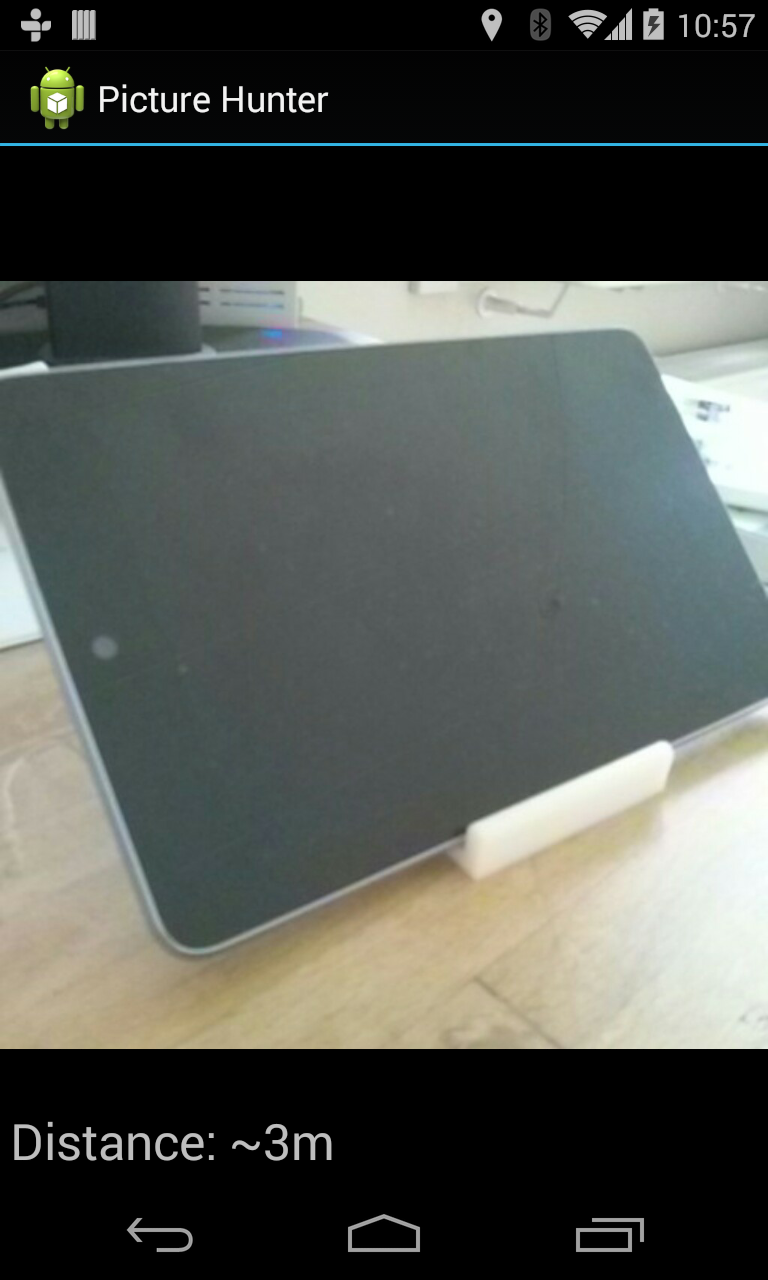
\includegraphics[width=0.3\textwidth]{img/detail}
		\caption{\label{fig:detail}Avståndet till där bilden togs visas tillsammans med bilden.}
	\end{figure}

	\begin{figure}[p]
		\centering
	    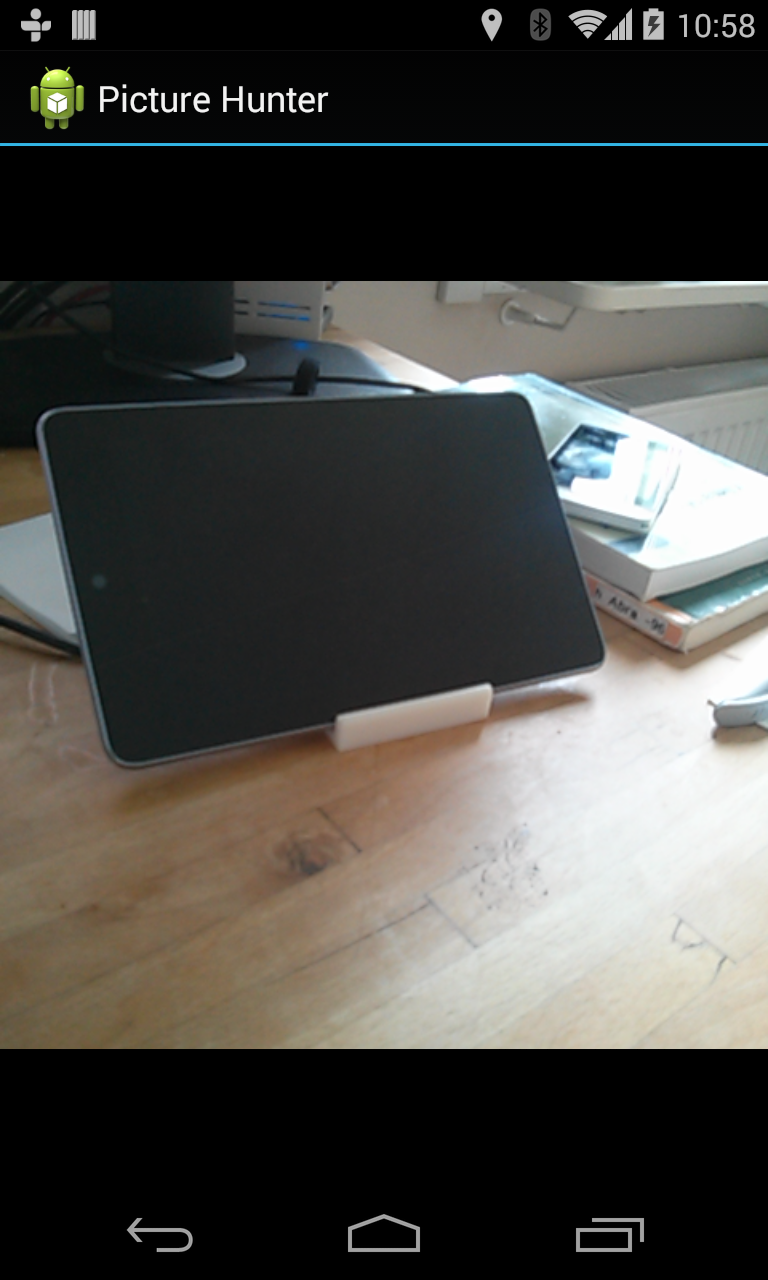
\includegraphics[width=0.3\textwidth]{img/camera}
		\caption{\label{fig:camera}Appen använder en specialutvecklad kamera.}
	\end{figure}

\subsection{Bildjämförelse}
	Bildjämförelsen består av två delar. Den första nås när användaren klickar på en omatchad bild och visar en större version av samma bild samt avståndet till vart bilden togs. Denna vy kan ses i figur \ref{fig:detail} Klickar man på bilden snurrar vyn (designprincip ``Delight me in surprising ways''\cite{Principles}) och på baksidan visas istället bilden från telefonens kamera (figur \ref{fig:camera}). Klickar man på kameravyn tas en bild, kameravyn stängs och den tagna bilden jämförs med referensbilden. Huruvida användaren lyckades matcha bilden meddelas med ett Toast-meddelande. Om användaren lyckades visas dessutom en ljusblå kryssruta uppe i högra hörnet. Kryssrutan kan även ses i miniatyrbilden när en bild är korrekt matchad.


\section{Teknik}

	Appen är uppbyggd med tre aktiviteter - en för album-vyn, en för bild-vyn och en för jämförelse.	Samtliga gränssnitt implementeras i huvudsak som fragment som i största möjliga mån är fristående från dess aktivitet. Vid behov används dock aktiviten som en mellanhand mellan fragmenten\cite{FragmentCommunication}. Ett tydligt exempel på detta är \emph{ComparisonActivity} som startar och avslutar de båda fragmenten efter vad som är lämpligt och som tar hand om bilden som kameran tagit.

	Appen uppvisar flera tekniska finesser. Några av dessa är ganska nyligen tillgada i Android så applikationen kräver en tämligen uppdaterad telefon. Den kräver även att telefonen har ett SD-kort, en kamera och NFC-förmåga.

\subsection{Bildigenkänning}
\label{subsec:image_recog}
	Den mest grundläggande funktionaliteten i appen är jämörelsen av två bilder. I början fanns förhoppningen att denna funkion skulle finnas i Androids api eller som ett externt bibliotek till java. Ingen av dessa möjligheter visade sig tyvärr möjliga varpå jag försökte mig på att implementera jämförelsen själv med hjälp av en post på \emph{Java Image Processing Cookbook}\cite{ImageComparison}.

	Jämförelsen görs genom att algoritmen väljer ut 100 punkter på varje bild och räknar ut den genomsnittsliga färgen i punktens omgivningen. Varje par punkter (en från varje bild) med samma position jämförs sedan var för sig och avståndet mellan färgerna i de två punkterna adderas till en total. Avstådet mellan två färger definieras i det här fallet som avstådet i ett tredimensionellt rum där röd, grön och blå utgör axlarna och med svart i origo. När det totala avståndet mellan bilderna räknats ut kan man jämföra detta med ett tröskelvärde som avgör hur mycket ``fel'' man tillåts. Enkelt uttryckt kan man alltså säga att algoritmen komprimerar bilden till 100x100 pixlar och sedan jämför färgen på bilderna för varje pixel.

	Det finns såklart flera problem med att bara jämföra färgvärden. Till exempel genererar endast stora förändringar i form ett betydande avstånd och små detaljer försvinner in i bakgrunden när bilden ``komprimeras''. Jämförelsen är också mycket känslig för olika ljusförhållanden. Att jämförelsen inte är exakt bör dock ses som en fördel då en viss grad av fel bör tillåtas för att jämförelsen ska vara praktiskt applicerbar. Skulle en liknande app byggas för kommersiellt bruk behöver man dock givetvis använda en mer avancerad algoritm.

\subsection{Kamera}
\label{subsec:camera}
	Då olika telefoner kan ta bilder i olika upplösning behövs någon standard införas på bilderna för att de ska kunna jämföras på ett rättvist sätt av algoritmen i avsnitt \ref{subsec:image_recog}. I vanliga fall skulle uppgiften att ta en bild delegeras till telefonens standardkameraapp men ett \emph{Intent} med \emph{ACTION\_IMAGE\_CAPTURE} har ingen möjlighet att påverka den slutliga storleken. Man hade kunnat normalisera bilden efteråt men då tar användaren en avlång bild men en liksidig sparas till disk. För att inte överraska användaren behöver kamerans bild motsvara slutresultatet. För att åstadkomma detta implementerades ett specialgjort kamerafragment. Kamerafragmentet används till all bildtagning i appen och begränsar bilderna till 1024x1024 pixlar.

\subsection{GPS}
	När en kameran i avsnitt \ref{subsec:camera} öppnas börjar appen fråga efter användarens koordinater. Om dessa funnits i tid till att bilden tas sparas dessa tillsammans med bilden som metadata och används för att ge spelaren som ska matcha bilden en idé om avståndet till platsen där bilden tagits.

\subsection{Near Field Communication (NFC)}
	För att dela bilder mellan två telefoner använder sig appen av Near Field Communication i from av \emph{Android Beam} (se figur \ref{fig:beam}). Överföring av filer med hjälp av Android Beam lades till först i api-nivå 16 vilket sätter detta som minimi-sdk-krav för att kunna använda appen. Så fort telefonen förs nära en annan (ca 4cm) kommer appen kontrollera om det finns bilder markerade. Dessa förs i så fall över till den andra telefonen och appen öppnas i så fall via ett speciellt Intent Filter. De nya filerna levereras sedan med hjälp av en \emph{Content Provider} som appen läser ifrån och flyttar in filerna till appens filarea.

	\begin{figure}[p]
		\centering
	    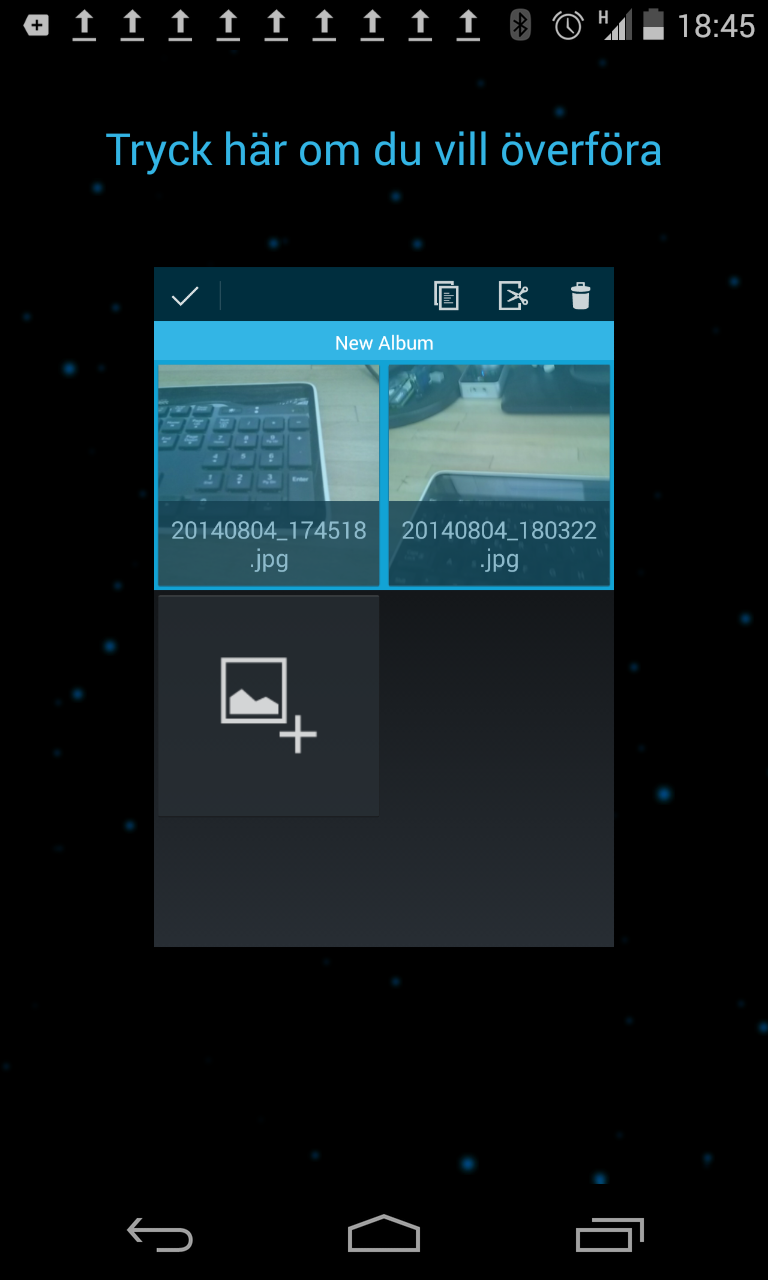
\includegraphics[width=0.3\textwidth]{img/beam}
		\caption{\label{fig:beam}Markerade filer kan överföras med Android Beam.}
	\end{figure}

\subsection{ViewPager}
\label{subsec:viewpager}
	ViewPager är ett ofärdigt\cite{ViewPager} men populärt api för lateral navigation. Vyn ska integreras i Androids normala api i framtiden men för tillfället finns en tidig version tillgänglig som en del av a \emph{android support library}.

\subsection{Animation}
	I appen finns en kort-vändnings-animation för bytet mellan den in-zoomade bildvyn och kameravyn. Animationen är specificerad i xml men använder det gamla animtionsbiblioteket istället för \emph{Animator} klasserna. Detta kommer sig av att \emph{Fragment}-klassen i supportbiblioteket, som måste användas i ViewPager:n från avsnitt \ref{subsec:viewpager}, inte stödjer det nya biblioteket\cite{SupportAnimator}. Av denna anledning är inte rotationen inte en ``riktig'' rotation utan istället är vyns skala i x-led animerad för att ge motsvarande intryck.

	Även en zoom-aninmation där minatyrbilden zoomades in och blev stor utvecklades (med animator biblioteket) och användes tidigt i projektet. Denna animation tvingades dock tas bort när den in-zoomade vyn byggdes om som ett eget fragment.

\subsection{Specialgjorda vyer och attribut}
	Två specialgjorda Views byggdes som en del i framtagandet av gränssnittet. Den ena är en fyrkantsvy som alltid är lika bred som hög. Man kan specificera i xml om den ska anpassa sig efter den tillgängliga höjden eller bredden. Denna funkionalitet kom till användning när appen behövde anpassas till landskapsläge.

	Den andra vy är en specialgjord layout som implementerar Checkable gränssnittet samt definierar ett extra drawable state för när vyn är ``kryssad''. Detta ger möjligheten att specificera bakgrunden med standard drawables. Vyn använder sig dessutom av ett semi-transparent lager som kan läggas in överst i layouten och därmed ge en färgförändring när vyn kryssas, trotts att bakgrunden täcks av andra komponenter. På detta sätt stödjer vyn användning både för album och bilder.

\subsection{Exif metadata}
	GPS datan som samplas in av kameran (avsnitt \ref{subsec:camera}) sparas som metadata i \emph{EXchangeable Image File}-format. För att kunna spara positionen i detta format behöver den först konverteras från decimal-format till timme/minut/sekund-format.

	Förutom gps-positionen sparas även om en bild har blivit matchad eller inte i bildens metadata. Androids förmåga att skriva Exif-data till en bild är ganska begränsad genom att endast vissa taggar stöds. På grund av detta skrivs matchnings-statusen till \emph{Model}-fältet istället.

\subsection{Backgrundsarbete och laddning}
	All bildhantering i appen är flyttat till bakgrundstrådar för att inte låsa gränssnittet\cite{BitmapProcessing}. Detta ses tydligast i listorna av bildminiatyrer där bilderna ibland dyker upp först efter en kort fördröjning. Dessutom undviker applikationen att ladda in stora bilder i minnet. Med hjälp av \emph{ThumbnailUtils} skapas miniatyrbilder i låg upplösning som låter appen hushålla bättre med sin minneskvota.



\section{Reflektion}
	Efter vad som föreföll en lång tids grubblande över vad för slags app jag ville bygga kom idén om att göra något med bildigenkänning. Efter lite sökning på nätet visade det sig finnas bibliotek som stödde denna funktion så jag kastade mig in i kodandet. Jag försökte visserligen stanna upp och sketcha ett par skärmar först, men jag blev snabbt otålig. Denna benägenhet till att inte definiera designen ordentligt tidigt i projektet är en svaghet i mitt arbetssätt som jag behöver arbeta mer på att förbättra. I huvudsak hade jag en bild av vad jag ville åstadkomma, och så här i efterhand kan jag säga att jag kom ganska nära.

	Kodandet skedde omväxlande med efterforskningar och gradvis växte applikationen fram. Då jag inte kommit i kontakt med flera komponenter i appen tidigare så gjordes många misstag. Hade jag haft kunskapen då som jag har nu hade det säkert gått betydligt snabbare. När jag läser koden kan jag se vilka delar som skrevs när i arbetet efter vilken lösning som valts eftersom jag hela tiden lärt mig och testat nya sätt att skriva koden.

	Överlag är jag nöjd med vad som åstadkommits och jag känner att jag lärt mig otroligt mycket på det här projektet.


\subsection{Säkerhet och etik}
	Appen är tämligen säker på så sätt att den inte använder sig av användarens information. Den ansluter inte till användarens konto och vet heller varken användarens namn, telefonnummer eller mail. Appen har bara tillgång till data som användaren avsiktligen ger den, dvs. bilder tagna med appens egna kamera.

	Bilder kan dock alltid vara kännsliga om de kommer på villovägar. Ponera att bilderna på något sätt kunde fångas av en tredje part. Då skulle hen ha tillgång till själva bilden, som kan avslöja vad användaren gjort vid tillfället eller med vem hen varit,  men även vart den tagits och därmed vart användaren befunnit sig. Det kan definitivt finnas anledningar till varför en person inte skulle vilja sprida den informationen.

	Förutom risken för oavsiktligt läckage kan användaren oroa sig för avsiktligt missanvändande av informationen som finns tillgänglig till appen. \emph{Picture Hunter} har inga onödiga rättigheter men har tillräckligt många och kraftfulla för att göra skada. Om appen på något sätt kunde ta bilder utan att användaren visste om det eller om appen periodiskt delade telefonens position med någon extern part skulle säkert inte användaren uppskatta detta. Delvis försvåras en sådan attack på användaren av att både användandet av gps och kamera måste synliggöras på telefonens gränssnitt.

	För att vissa telefonen ska kunna ta bilder måste telefonen vara upplåst och bilderna från kameran måste visas på skärmen i en \emph{SurfaceView}. Det finns dock inga storleksrestriktioner på denna vy, så det räcker med att den renderas på en pixel vilket kan göra den praktiskt oigenkännbar. För gps:en är det mer möjligt att hämta data dolt. När gps:en är igång visas en ikon i statusranden överst i gränssnittet, men den är lätt att missa. Appen kan dessutom välja att hämta positionen medans telefonen sover via en \emph{Service} i bakgrunden.

	En trygghet som användaren har när hen tänker på frågorna diskuterade ovan är att appen inte har några möjligheter att använda internet. Så även om appen samlar information om användaren finns inga uppenbara möjligheter att föra vidare den till en extern part. En mer omständig möjlighet finns dock. Kan man få användaren att installera två appar, en med internet och sd-kort tillgång men inget annat, samt en app med tillgång till flera sensorer och tjänster, inklusive sd-kortet, men inte internet, kan man använda sd-kortet för att kommunicera mellan apparna och därmed sprida datan.

	En sista fara som användaren kan tänkas vara rädd för är om appen skickar data till en annan telefon som den inte bör. Eftersom appen begär tillgång till hela sd-kortet kan också skicka vilken fil som helst därifrån till andra telefoner den kommer i kontakt med via NFC. Lyckas appen då hitta användarens nakenbilder eller kanske hemliga ritningar från jobbet och skicka dessa blir nog inte användaren så glad. Det är dock svårt att se hur appens skapare skulle tjäna på ett sådant beteende.

	Allt eftersom fler ``features'' läggs till i apparna kräver de också fler tillåtelser som användaren kommer ha svårt att tacka nej till. Även om användaren litar på appens skapare kanske rättigheterna till appen säljs till ett annat företag som inte har lika rena avsikter. I slutändan måste användaren lita på skaparen av appen, för även med få och till synes oskyldiga tillåtelser kan man åsamka skada och ställa till problem om de används i detta syfte. Användaren får helt enkelt försöka undvika uppenbart problematiska appar och kan bara hoppas att någon annan råkar ut för problem och anmäler övriga appar med ont uppsåt.


\subsection{Förbättringar och vidare arbete}

	Om jag hade byggt en ny version av appen hade jag slagit ihop \emph{AlbumListActivity/PhotoListActivity} och \emph{AlbumListFragment/PhotoListFragment} till en ända aktivitet respektive fragment. Detta skulle kännas snyggare, men uppdelningen hjälper faktiskt till att separera vad som ska hända vid användarinteraktion. Genom att gemensam kod har extraherats till egna klasser dupliceras dessutom kod endast marginellt. Med detta i åtanke har jag fokuserat på andra delar av appen och inte refaktorerat om då jag befarar att det skulle ta en ansenlig tid och inte ge så mycket ``poäng'' i kursen. För kursens skull hoppas jag det kan räcka med att visa att jag är medveten om problemet.

	Ifall appen skulle släppas till allmänheten skulle det krävas mer ``hints'' till användaren om hur hen ska använda appen. I dagsläget förklaras få saker i appen och det finns t.ex. inte någon knapp för att ta bilder - vilket antagligen varit tydligare (om än inte funktionellt bättre). Då jag inte ämnar släppa applikationen har jag inte prioriterat upplärning av användare men har försökt använda standardiserade interaktioner.

	Om appen släpps till allmänheten är det möjligt att ett mer prfilerat gränssnitt hade varit lämpligt. Appen är byggd för att vara så transparent som möjligt men som marknadsföring är detta troligen ett dåligt drag eftersom igenkänningen minskar. Gladare färger kan också tänkas attrahera användare bättre när de ser appen för första gången.

	I dagsläget är enda möjligheten till bildöverföring NFC. Detta kräver att båda parter fysiskt träffas för att föra över bilder. Man kan lätt föreställa sig ett scenario där spelarna vill överföra bilder via MMS eller liknande. I en framtida app borde man kunna dela bilderna som vilken fil som helst.

	En sista förbättring skulle kunna vara att byta bildjämförelsealgoritm då den nuvarande är ganska naiv och känslig. En bättre algoritm skulle kunna tänkas normalisera färgerna eller jobba med kant-identifiering.



\begingroup
\raggedright
\bibliographystyle{plain}
\bibliography{references}
\addcontentsline{toc}{section}{Referenser}
\endgroup

\end{document}